% Use only LaTeX2e, calling the article.cls class and 12-point type.

\documentclass[12pt]{article}

% Users of the {thebibliography} environment or BibTeX should use the
% scicite.sty package, downloadable from *Science* at
% www.sciencemag.org/about/authors/prep/TeX_help/ .
% This package should properly format in-text
% reference calls and reference-list numbers.

\usepackage{scicite}

% Use times if you have the font installed; otherwise, comment out the
% following line.

\usepackage{times}

\usepackage{graphicx}% Include figure files

% The preamble here sets up a lot of new/revised commands and
% environments.  It's annoying, but please do *not* try to strip these
% out into a separate .sty file (which could lead to the loss of some
% information when we convert the file to other formats).  Instead, keep
% them in the preamble of your main LaTeX source file.


% The following parameters seem to provide a reasonable page setup.

\topmargin 0.0cm
\oddsidemargin 0.2cm
\textwidth 16cm 
\textheight 21cm
\footskip 1.0cm

\newcommand{\asy}{A}               % raw uncorrected asymmetry
\newcommand{\acorr}{A^{\rm corr}}  % asymmetry with additive corrections
\newcommand{\aexp}{A^{\rm exp}}    % asymmetry with polarization correction
\newcommand{\aphys}{A^{\rm phys}}  % asymmetry with all corrections
\newcommand{\apv}{A^{\rm PV}}      % theoretical asymmetry
\newcommand{\ath}{A^{\rm th}}      % analyzing power
\newcommand{\af}{A_{{F}}}
\newcommand{\pg}{P_{\gamma}}
\newcommand{\etal}{\it et.al}

%The next command sets up an environment for the abstract to your paper.

\newenvironment{sciabstract}{%
\begin{quote} \bf}
{\end{quote}}


% If your reference list includes text notes as well as references,
% include the following line; otherwise, comment it out.

\renewcommand\refname{References and Notes}

% The following lines set up an environment for the last note in the
% reference list, which commonly includes acknowledgments of funding,
% help, etc.  It's intended for users of BibTeX or the {thebibliography}
% environment.  Users who are hand-coding their references at the end
% using a list environment such as {enumerate} can simply add another
% item at the end, and it will be numbered automatically.

\newcounter{lastnote}
\newenvironment{scilastnote}{%
\setcounter{lastnote}{\value{enumiv}}%
\addtocounter{lastnote}{+1}%
\begin{list}%
{\arabic{lastnote}.}
{\setlength{\leftmargin}{.22in}}
{\setlength{\labelsep}{.5em}}}
{\end{list}}


% Include your paper's title here

\title{PVDIS Supplemental Material - Measurement of the Parity Violating
Deep Inelastic Asymmetry and Extraction of the Quark Weak Axial Charge} 


% Place the author information here.  Please hand-code the contact
% information and notecalls; do *not* use \footnote commands.  Let the
% author contact information appear immediately below the author names
% as shown.  We would also prefer that you don't change the type-size
% settings shown here.

\author{
D.~Wang,$^{1}$  K.~Pan,$^{2}$  R.~Subedi,$^{1}$  X.~Deng,$^{1}$  Z.~Ahmed,$^{4}$  K.~Allada,$^{5}$  \\
K.~A.~Aniol,$^{6}$  D.~S.~Armstrong,$^{7}$  J.~Arrington,$^{8}$  V.~Bellini,$^{9}$  R.~Beminiwattha,$^{10}$  \\
J.~Benesch,$^{11}$  F.~Benmokhtar,$^{12}$  A.~Camsonne,$^{11}$  M.~Canan,$^{13}$  G.~D.~Cates,$^{1}$  \\
J.-P.~Chen,$^{11}$  E.~Chudakov,$^{11}$  E.~Cisbani,$^{14}$  M.~M.~Dalton,$^{1}$  C.~W.~de~Jager,$^{11,1}$  \\
R.~De Leo,$^{15}$  W.~Deconinck,$^{7}$  A.~Deur,$^{11}$  C.~Dutta,$^{5}$  L.~El~Fassi,$^{8}$  D.~Flay,$^{16}$  \\
G.~B.~Franklin,$^{12}$  M.~Friend,$^{12}$  S.~Frullani,$^{14}$  F.~Garibaldi,$^{14}$  A.~Giusa,$^{9}$  \\
A.~Glamazdin,$^{17}$  S.~Golge,$^{13}$  K.~Grimm,$^{18}$  K.~Hafidi,$^{8}$  O.~Hansen,$^{11}$  D.~W.~Higinbotham,$^{11}$  \\
R.~Holmes,$^{4}$  T.~Holmstrom,$^{19}$  R.~Holt,$^{8}$  J.~Huang,$^{2}$  C.~E.~Hyde,$^{13,20}$  C.~M.~Jen,$^{4}$  \\
D.~Jones,$^{1}$  H.~Kang,$^{21}$  P.~King,$^{10}$  S.~Kowalski,$^{2}$  K.~S.~Kumar,$^{22}$  J.~H.~Lee,$^{7,10}$  \\
J.~J.~LeRose,$^{11}$  N.~Liyanage,$^{1}$  E.~Long,$^{23}$  D.~McNulty,$^{22}$  D.~Margaziotis,$^{6}$  F.~Meddi,$^{14}$  \\
D.~G.~Meekins,$^{11}$  L.~Mercado,$^{22}$  Z.-E.~Meziani,$^{16}$  R.~Michaels,$^{11}$  M.~Mihovilovic,$^{24}$  \\
N.~Muangma,$^{2}$  K.~E.~Myers,$^{4}$  S.~Nanda,$^{11}$  A.~Narayan,$^{25}$  V.~Nelyubin,$^{1}$  Nuruzzaman,$^{25}$  \\
Y.~Oh,$^{21}$  D.~Parno,$^{12}$  K.~D.~Paschke,$^{1}$  S.~K.~Phillips,$^{26}$  X.~Qian,$^{27}$  \\
Y.~Qiang,$^{27}$  B.~Quinn,$^{12}$  A.~Rakhman,$^{4}$  P.~E.~Reimer,$^{8}$  K.~Rider,$^{19}$  S.~Riordan,$^{1}$  \\
J.~Roche,$^{10}$  J.~Rubin,$^{8}$  G.~Russo,$^{9}$  K.~Saenboonruang,$^{1}$  A.~Saha,$^{11},\dagger$, B.~Sawatzky,$^{11}$  \\
A.~Shahinyan,$^{11}$  R.~Silwal,$^{1}$  S.~Sirca,$^{24}$  P.~A.~Souder,$^{4}$  R.~Suleiman,$^{11}$  V.~Sulkosky,$^{2}$  \\
C.~M.~Sutera,$^{9}$  W.~A.~Tobias,$^{1}$  B.~Waidyawansa,$^{10}$  B.~Wojtsekhowski,$^{11}$  L.~Ye,$^{28}$  B.~Zhao,$^{7}$  \\
X.~Zheng,$^{1,\ast}$\\
\\
\normalsize{$^{1}$University of Virginia, Charlottesville, Virginia 22904, USA} \\
\normalsize{$^{2}$Massachesetts Institute of Technology, Cambridge, MA 02139, USA}\\
\normalsize{$^{3}$George Washington University, Washington, District of Columbia 20052, USA}\\
\normalsize{$^{4}$Syracuse University, Syracuse, New York 13244, USA}\\
\normalsize{$^{5}$University of Kentucky, Lexington, Kentucky 40506, USA}\\
\normalsize{$^{6}$\mbox{California State University, Los Angeles}, Los Angeles, California 90032, USA}\\
\normalsize{$^{7}$College of William and Mary, Williamsburg, Virginia 23187, USA}\\
\normalsize{$^{8}$Physics Division, Argonne National Laboratory, Argonne, Illinois 60439, USA}\\
\normalsize{$^{9}$Istituto Nazionale di Fisica Nucleare, Dipt.~di Fisica dell'Univ.~di Catania, I-95123 Catania, Italy}\\
\normalsize{$^{10}$Ohio University, Athens, Ohio 45701, USA}\\
\normalsize{$^{11}$Thomas Jefferson National Accelerator Facility, Newport News, Virginia 23606, USA}\\
\normalsize{$^{12}$Carnegie Mellon University, Pittsburgh, Pennsylvania 15213, USA}\\
\normalsize{$^{13}$Old Dominion University, Norfolk, Virginia 23529, USA}\\
\normalsize{$^{14}$INFN, Sezione di Roma, gruppo Sanit\`a and Istituto Superiore di Sanit\`a, I-00161 Rome, Italy}\\
\normalsize{$^{15}$Universit\`a di Bari, I-70126 Bari, Italy}\\
\normalsize{$^{16}$Temple University, Philadelphia, Pennsylvania 19122, USA}\\
\normalsize{$^{17}$Kharkov Institute of Physics and Technology, Kharkov 61108, Ukraine}\\
\normalsize{$^{18}$Louisiana Technical University, Ruston, Louisiana 71272, USA}\\
\normalsize{$^{19}$Longwood University, Farmville, Virginia 23909, USA}\\
\normalsize{$^{20}$Clermont Universit\'e, Universit\'e Blaise Pascal, CNRS/IN2P3,
Laboratoire de Physique Corpusculaire, FR-63000 Clermont-Ferrand, France}\\
\normalsize{$^{21}$Seoul National University, Seoul 151-742, South Korea}\\
\normalsize{$^{22}$University of Massachusetts Amherst, Amherst, Massachusetts 01003, USA}\\
\normalsize{$^{23}$Kent State University, Kent, Ohio 44242, USA} \\
\normalsize{$^{24}$Institut Jo\v zef Stefan, 3000 SI-1001 Ljubljana, Slovenia}\\
\normalsize{$^{25}$Mississippi State University, Starkeville, Mississippi 39762, USA}\\
\normalsize{$^{26}$University of New Hampshire, Durham, New Hampshire 03824, USA}\\
\normalsize{$^{27}$Duke University, Durham, North Carolina 27708, USA}\\
\normalsize{$^{28}$China Institute of Atomic Energy, Beijing, 102413, P. R. China}\\\\
%
\normalsize{$^\dagger$Deceased}
\normalsize{$^\ast$To whom correspondence should be addressed; E-mail: xiaochao@jlab.org}
%
}

% Include the date command, but leave its argument blank.

\date{}


%%%%%%%%%%%%%%%%% END OF PREAMBLE %%%%%%%%%%%%%%%%



\begin{document} 

% Double-space the manuscript.

\baselineskip24pt

% Make the title.

\maketitle 



% Place your abstract within the special {sciabstract} environment.

\begin{sciabstract}
In this document we provide supplemental material in support of ... ...

\end{sciabstract}

%PVDIS Formalism
\section{PVDIS Formalism}\label{sec:formalism}

This section discusses the formalism of parity-violating deep inelastic
scattering.  Extraction of the $C_2$ coefficients (section ~\ref{sec_2coeff}) 
follow from this formalism.

%
\begin {eqnarray}
%A_{PV}  &=& \frac{\sigma_{+} - \sigma_{-}}{\sigma_{+} + \sigma_{-}}\nonumber\\
%&=&(\frac{3G_FQ^2}{\pi \alpha^2 \sqrt{2}})(\frac{1}{5+R_S(x)+4R_C(x)})\nonumber\\
%&&\times\left\{2C_{1u}[1+R_C(x)]-C_{1d}[1+R_S(x)]+\right.\nonumber\\ 
%&&~~~\left.Y({2C_{2u}-C_{2d}})R_V(x)\right\}~,
A_{PV}  &\equiv& \frac{\sigma_{+} - \sigma_{-}}{\sigma_{+} + \sigma_{-}}
=\left(-\frac{G_FQ^2}{4\sqrt{2}\pi \alpha}\right)
  \left(2g_A^e Y_1\frac{F_1^{\gamma Z}}{F_1^\gamma}+{g_V^e}Y_3\frac{F_3^{\gamma Z}}{F_1^\gamma}\right)~,
%&&\times\left\{2C_{1u}[1+R_C(x)]-C_{1d}[1+R_S(x)]+\right.\nonumber\\
%&&~~~\left.Y({2C_{2u}-C_{2d}})R_V(x)\right\}~,
\end{eqnarray}
where $Q^2$ is the negative of the 
four-momentum transfer squared, $G_F$ is the Fermi weak coupling constant, 
$\alpha$ is the fine structure constant, $Y_1$ and $Y_3$ are kinematic factors,
and $x$ is the Bjorken scaling variable. %
%(for details see Ref.~\cite{PR05-007,PR08-011}),
In the quark parton model,
\begin{eqnarray}
 F_1^{\gamma Z} &=& \sum{g_V^q Q_q\left[q(x) + \bar q(x)\right]} \\
 F_3^{\gamma Z} &=& \sum{g_A^q Q_q\left[q(x) - \bar q(x)\right]} \\
 F_1^{\gamma} &=& \frac{1}{2}\sum{Q_q^2\left[q(x) + \bar q(x)\right]}
\end{eqnarray}
where $Q_q$ is the electric charge of quarks and 
$q(x)$, $\bar q(x)$ are quark distribution functions.
Rewriting $g_{A(V)}^e g_{V(A)}^q$ as $C_{1(2)q}$, and assuming
$R^\gamma = R^{\gamma Z} = 0$, one has $Y_1=1$ and
\begin {eqnarray}
 A_{PV} &=&\left(\frac{3G_FQ^2}{\pi \alpha^2 \sqrt{2}}\right)\times \nonumber\\
 && \frac{2C_{1u}[1+R_C(x)]-C_{1d}[1+R_S(x)]+Y_3(2C_{2u}-C_{2d})R_V(x)}{5+R_S(x)+4R_C(x)}~,
\end{eqnarray}
%
where $R_{V,C,S}$ are related to quark distributions.
The magnitude of the asymmetry is in the order of $10^{-4}$, or $10^2$~parts per million
(ppm) at $Q^2=1$~(GeV/$c$)$^2$.


The tree-level Standard Model effective weak coupling constants $C_{1,2q}$ are
\begin{eqnarray}
 C_{1u} = 2g^e_A g^u_V= -\frac{1}{2} + \frac{3}{4} \sin^2\theta_{W}~,
 && ~C_{2u} = 2g^e_V g^u_A= - \frac{1}{2} + 2 \sin^2\theta_{W}~,\nonumber\\
 C_{1d} = 2g^e_A g^d_V= \frac{1}{2} - \frac{2}{3} \sin^2\theta_{W}~,
 && ~C_{2d} = 2g^e_V g^d_A=  \frac{1}{2} - 2 \sin^2\theta_{W}~,\nonumber
\end{eqnarray}
with $\theta_W$ the weak mixing angle. 
The goal of JLab E08-011 is to measure the PVDIS asymmetries to a statistical precision of 
3\% for the $Q^2 = 1.1 {\rm GeV}^2$ point and 4\% for the the $Q^2 = 1.9 {\rm GeV}^2$ point.
In addition, the systematic uncertainty goal is $<3\%$, 
and under the assumption that hadronic physics corrections are small, 
our goal is to extract from these asymmetries the effective coupling 
constant combination $(2C_{2u} - C_{2d})$. 
The magnitude of the asymmetries is expected to be $90$ and $170$~ppm for the two
measured kinematics of $Q^2=1.1$ and $1.9$~(GeV/$c$)$^2$, respectively. 
To achieve the required precision, event rates up to $500$~kHz are expected.
%
Although this is not the first time the PVDIS asymmetries are measured, the only
preceeding PVDIS measurement was carried out at SLAC~\cite{Prescott:1978tm,Prescott:1979dh}
about 35 years ago, with a $\approx 9$\% statistical and a $\approx 9$\% systematic uncertainties. 
The increased precision of this experiment required better controls of all systematic
uncertainties.

%Apparatus

\section{Apparatus}\label{sec:apparatus}

\par The experimental techniques for measuring small 
asymmetries of order 1 ppm have been successfully deployed in
parity experiments at electron
scattering facilities \cite{SLAC}-\cite{happex}.
The recent experiments at Jefferson Lab, such as HAPPEX ~\cite{happex}
and PREX ~\cite{prex} have maintain systematic errors associated with helicity
reversal at the $10^{-8}$ level.
The asymmetries sought for in this experiment are of order 100 ppm with
accuracies of about 1 ppm, which is two orders-of-magnitude above the 
established systematic error.

A significant challenge of the measurement 
is to separate electrons from the charged pion background that arise from electro- or photo-productions. 
While the standard HRS detector package and data acquisition (DAQ) system routinely provide 
such a high particle identification (PID) performance, they are based on full recording 
of the detector signals and are limited to event rates up to 4 kHz.
This is not sufficient for the few-hundred kHz rates for the experiment. 
Thus we have built new DAQ designed to count event rates up to 1~MHz with hardware-based 
particle identification ~\cite{pvdis_nim}.

The main parts of the apparatus will be described in this section.
These include the polarized electron beam, the beam monitors, the spectrometers
and detectors, the data acquisition system, and the beam polarimeters.


\subsection{Polarized Electron Beam}\label{sec:app_electronbeam}

The electron beam originated from a strained GaAsP 
photocathode illuminated by 
circularly polarized light~\cite{Sinclair2007}.
The sign of the laser polarization determined the electron
helicity; this was held constant for periods of 33 msec,
referred to as ``windows''.
By reversing the sign of the laser circular 
polarization, the direction of the spin at the target could be 
reversed rapidly \cite{Paschke:2007zz}.
Two windows of opposite helicity made a window pair, where
the helicity of the first window was chosen with a pseudorandom
number generator and the second window was the complement.
These window pairs were line locked to the 60 Hz line,
thus ensuring a good cancellation of the power-line noise. 
 
A half-wave ($\lambda$/2) plate was periodically inserted into the 
laser optical path which passively reversed the
sign of the electron beam polarization. 
Roughly equal statistics were thus 
accumulated with opposite signs for the measured asymmetry, 
which suppressed many systematic effects.  
The direction of the polarization could also be
controlled by a Wien filter and solenoidal lenses
near the injector \cite{GramesWien2011}.  The accelerated beam was 
directed into Hall A, where its intensity, energy and trajectory on 
target were inferred from the response of several monitoring devices.

The beam monitors and trigger signals, which derived from
the detectors in the spectrometers, 
were integrated over the helicity window
and digitized.  The beam monitors were integrated by
custom 18-bit ADCs ~\cite{ref:prex}, while the
trigger signals for electrons and pions were integrated
in scalers from trigger signals that were generated by a NIM-based
trigger and DAQ system ~\cite{ref:pvdis_nim} (see sec ~\ref{sec:daq}).
The beam monitors, target, and detectors were
designed so that
the fluctuations in the fractional difference in 
the signal response between
a pair of successive windows were
dominated by scattered electron counting statistics.
To keep spurious beam-induced asymmetries under
control at well below the ppm level, 
careful attention was given to the design and configuration of the laser 
optics leading to the photocathode \cite{Paschke:2007zz}.

The integrated response of each detector PMT and beam monitor
was digitized and recorded for each 33 msec window.
The raw spin-direction asymmetry $A_{raw}$
in each spectrometer arm was computed from the the detector response
normalized to the beam intensity 
for each window pair. 


\subsection{Beam Monitoring}
\label{sec:beam_mon}

Helicity-correlations in the beam properties such as energy and position are
a primary concern for parity-violation experiments.  
At Jefferson Lab, the beam position is measured by ``stripline"
monitors~\cite{stripline}, each of which consists of a set of four thin wires
placed symmetrically around the beam pipe. The wires act as antennae
that provide a signal (modulated by the microwave structure of the
electron beam) proportional to the beam position as well as
intensity. Figure~\ref{fig5:jlabcorr} shows the correlation between
the measured position at a BPM near the target compared with the
predicted position using neighboring BPMs for a beam current of
100 $\mu$A ($2\times 10^{13}$ electrons per window). A precision
for $\delta(\Delta X_i)$ close to 1 $\mu$m was obtained for the
average beam position for a beam window containing $2\times
10^{13}$ electrons.

\begin{figure}[tb]
\begin{center}
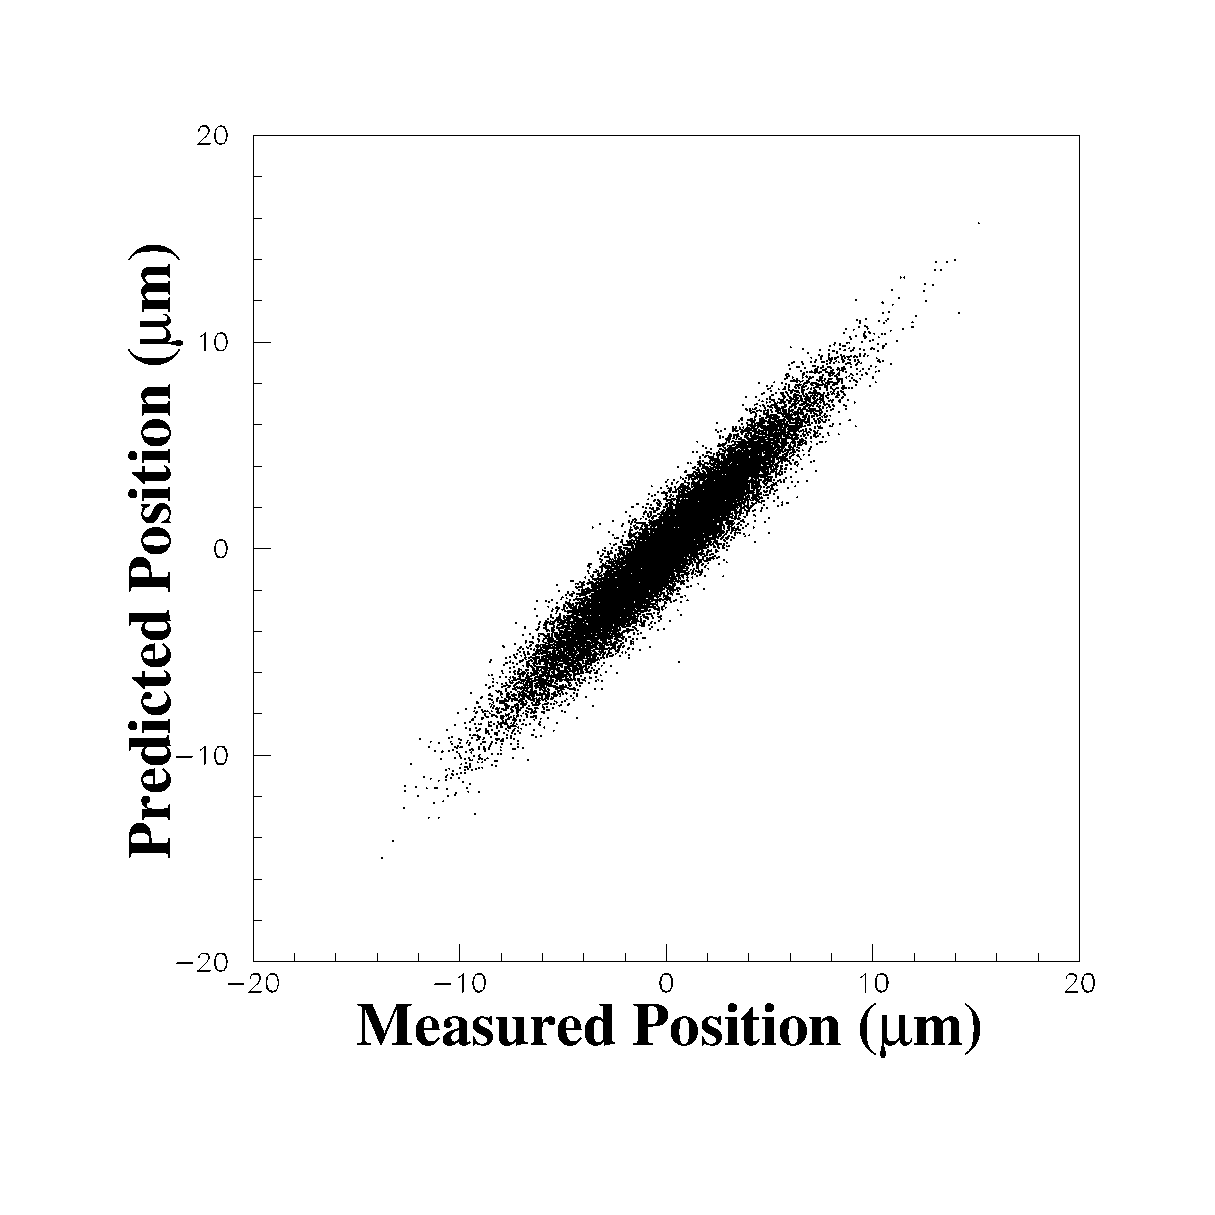
\includegraphics[width=3.6in]{RM/fig5_ycorrbw.eps}
\caption{Window-to-window beam jitter as measured
by a BPM is 
plotted along the $x$ axis. On the $y$ axis is plotted the beam
position as predicted by nearby BPMs. The residuals are smaller
than 1 $\mu$m.}
\label{fig5:jlabcorr}
\end{center}
\end{figure}

To measure the beam intensity, microwave cavity BCMs have been
developed at Jefferson Lab~\cite{A-NIM}. The precision $\delta(\asy_I)$ that has
been achieved for a 30 ms beam window at 100 $\mu$A is $4\times
10^{-5}$. This superior resolution is a 
result of good radiofrequency (rf)
instrumentation as well as a high resolution 18-bit ADC, which
will be discussed in section \ref{sec:daq}.

Let the detected scattered flux of electrons be $D$ in each spectrometer,
and the beam current $I$,
measured independently for every window
by integrating the signals over the helicity period.  From these 
we obtained the normalized flux $d_i \equiv D_i/I_i$ and 
the cross section asymmetry $(A_d)_i$ for the
$i$th window pair. The raw asymmetry was then obtained by
appropriate averaging of $N$ measurements:
%
\begin{eqnarray} \label{eq:asyraw}
(A_d)_i & \equiv &
{\left(\frac{d^+-d^-}
{d^++d^-}\right)}_i 
\equiv {\left(\frac{\Delta d}
{2d}\right)}_i 
\nonumber \\
\quad \delta(\asy_d) & = &
\sigma(\asy_d)/\sqrt{N}. \label{eqn:pulsepair}
\end{eqnarray}
%
where $+$ and $-$ denote the two helicity states in a pair.

A major goal of the experimental design is to $\sigma(\asy_d)$ should be
dominated by the counting statistics in the scattered flux.
As shown by fig N in ref ~\cite{pvdis_nim}, this goal was met.

There are two key parameters for each experimentally measured
quantity $M$, such as detector rate, beam intensity, or beam position. 
The first is $\sigma(\Delta M)$, the size of the relative window pair-to-window pair
fluctuations in $\Delta M\equiv M_{+} - M_{-}$, which is affected by
real fluctuations in the electron flux. The second is
$\delta(\Delta M)$, the relative accuracy with which the window
pair differences in $M$ can be measured compared to the true
value, which is dominated by instrumentation noise.

If $\sigma(\Delta M)$ is large enough, it might mean that there
are non-statistical contributions to $\sigma(\asy_d)$ so that the
latter is no longer dominated by counting statistics. In this
case, it is crucial that $\delta(\Delta M)\ll\sigma(\Delta M)$ so
that window pair to window pair corrections for the fluctuations
in $\Delta M$ can be made.

As stated in \ref{sec:beam_fluc}, we desire that
$\sigma(\asy_d)$ be dominated by counting statistics.
An example of possible non-statistical contributions
is window-to-window relative beam intensity
fluctuations, $\sigma(A(I)) \equiv \sigma(\Delta I/2I)$,
which were observed to vary between $2\times 10^{-4}$ and
$2\times 10^{-3}$, depending on the quality of the laser and the
beam tune. This is remarkable and a unique feature of the beam at
Jefferson lab, since $\sigma(\asy_I)<\sigma(\asy_d)$. Nevertheless, the
detector-intensity correlation can be exploited to remove the
dependence of beam charge fluctuations on the measured asymmetry:
\begin{equation}
(\asy_d)_i \simeq
\left(\frac{\Delta D}{2D} - \frac{\Delta I}{2I}\right)_i \equiv
(\asy_D - \asy_I)_i.
\end{equation}
(This is equation \ref{eq:asyraw}
to first order.)

Similarly, $\sigma(\asy_d)$ might be affected by random beam
fluctuations in energy, position and angle. The corrections can be
parameterized as follows:
\begin{equation}
(\acorr_d)_i = \left(\frac{\Delta D}{2D} - \frac{\Delta I}{2I}\right)_i
-\sum_j{\left( {\alpha_j(\Delta X_j)_i}\right)}.
\end{equation}
Here, $X_j$ are beam parameters such as energy, position and
angle and $\alpha_j \equiv \partial D/\partial X_j$ are
coefficients that depend on the kinematics of the specific
reaction being studied, as well as the detailed spectrometer and
detector geometry of the experiment.

By judicious choices of beam position monitoring devices (BPMs)
and their respective locations, several measurements of beam
position can be made from which the average relative energy,
position, and angle of approach of each ensemble of electrons in a
helicity window on target can be inferred. One can then write
\begin{equation} 
(\acorr_d)_i = \left(\frac{\Delta D}{2D} - \frac{\Delta I}{2I}\right)_i
-\sum_j{\left({\beta_j(\Delta M_j)_i}\right)}.
\end{equation}
Here $M_i$ are a set of 5 BPMs that span the parameter space of
energy, position, and angle on target, and $\beta_i \equiv \partial
D/\partial M_i$. It is worth noting that this approach of making
corrections window by window automatically accounts for occasional
random instabilities in the accelerator (such as klystron
failures) that are characteristic of normal running conditions.

During our experiment run, we found that $\sigma(\Delta M_j)$ varied
between 1 and 10 $\mu$m and $\sigma (\asy_E)$ was typically less
than $10^{-5}$. These fluctuations were small enough that their
impact on $\sigma (\asy_d)$ was negligible. Indeed, we believe that a
significant contribution to the fluctuations in each monitor
difference $\Delta M$ was the intrinsic measurement precision
$\delta(\Delta M_i)$. We elaborate on this in section
~\ref{sec:beam_mon},
where we discuss the monitoring instrumentation.

Another important consideration is the accuracy with which the
coefficients $\beta_i$ are measured. As mentioned earlier, these
coefficients were evaluated using beam modulation, and will be
discussed in Sect.~\ref{bmod}.

The above discussion regarding measurement accuracy and its impact
on $\sigma(\asy_d)$ is particularly relevant in the monitoring of the
electron beam properties such as beam intensity, trajectory and
energy.

\subsection{Spectrometers and Detectors}\label{sec:HRS}

The Hall A high resolution spectrometers (HRS) at
Jefferson Lab consist of a pair
of identical spectrometers of QQDQ design,
together with detectors for detecting the 
scattered particles \cite{A-NIM}.
The spectrometer and their standard detector 
package served to select for and to 
measure the kinematics quantities ($x, Q^2$)
while suppressing backgrounds originating
from the target.

\par
The spectrometers are designed to have a
large acceptance with excellent 
resolution ($\Delta E / E \sim 10^{-4}$)
and absolute accuracy
in the reconstructed
four--vectors of the events and, 
of less relevance for our experiment,
precise normalization of the cross section.
To measure $Q^2$ with sufficient accuracy
requires good knowledge of the transfer matrix for
the spectrometer to reconstruct events at the
scattering point, as well as
good pointing accuracy for the location of the
spectrometers and precise measurements 
of beam position and angle.
To calibrate the transfer matrix, a 0.5 mm thick 
tungsten plate with an array of pinholes
is inserted in dedicated runs; reconstruction
of the hole pattern determines the matrix.

The scattered rate of electrons and of pions were 
determined by a trigger system
in the HRS described in ~\cite{pvdis_nim}.
This trigger consisted of two scintillator planes, which provided
the main timing trigger, a CO$_2$ gas cherenkov counter and a 
double-layered lead glass 
detector, which both provided particle identification information. 
The standard tracking detector (the vertical 
drift chamber) was turned off during production data 
taking because it may not endure
the expected high event rates. 
During low-rate calibration runs, the tracking detector 
was turned on and the efficiency of the electron trigger 
and the pion rejection could be studied (see ref ~\ref{pvdis:nim}).

The signals for
the gas cherenkov detector and the double-layered lead glass counter
were passed through discriminators and logic units to form 
preliminary electron and pion triggers. 
These preliminary triggers are then combined with the 
scintillator triggers and cherenkov 
signals to form the final electron and pion triggers, which are then 
sent to scalers to record the event counts and form asymmetries.  
Particle identification 
is fulfilled by the use of discriminators for both the lead-glass 
and the cherenkov counters 
and proper settings of their thresholds. 

For HRS the two layers of the leadglass counter are 
called ``preshower'' and ``shower'' detectors, 
respectively. The preshower blocks in the Right HRS 
(the spectrometer located to the right 
side of the beamline when viewed along the beam direction) 
has $48$ blocks arranged in a $2\times 24$ 
array, with the longest dimension of the 
blocks aligned perpendicular to the particle trajectory. For the two blocks
in each row, only the ends facing outward are read 
out by photo-multiplier tubes (PMTs) and 
the other ends of the two blocks were facing each other 
and not read out. Therefore the 
preshower detector had $48$ output channels. All preshower 
blocks were individually wrapped 
to prevent light leak. The preshower and the shower detectors 
in the Left HRS are similar to 
the preshower detector on the Right HRS except that for each 
detector there are $34$ blocks 
arranged in a $2\times 17$ array. The shower detector in the 
Right HRS had $75$ blocks 
arranged in a $5\times 15$ array with the longest dimension 
of the blocks aligned along the trajectory of 
scattered particles. PMTs are attached to each block of 
the Right shower detector on one end only, 
giving $75$ output channels.

The particle identification (PID) was studied at 
low beam currents using 
fbTDC signals along with ADC spectrum
of all detector signals recorded by the standard DAQ. 
Figure~\ref{fig:showerspectrum} shows the preshower vs. shower
signals for group 2 on the Left HRS. A comparsion between no fbTDC cut and with 
cut on the fbTDC signal of the electron wide trigger from this group clearly shows the 
hardware PID cuts.
%
\begin{figure}[!ht]
\hspace*{0.8cm}
\includegraphics[width=0.9\textwidth]{epsFig/run_22060_group2_PSvsSH_edit.eps}
\hspace*{-0.2cm}
\caption{Preshower vs. Shower ADC spectrum (sum of 8 blocks each) for group 2 on the Left HRS,
without fbTDC cut (left) and with cut on the group 2 electron wide trigger fbTDC
signal (right). It clearly shows the hardware cuts on the preshower and the total
shower signals, indicating the DAQ is selecting the correct events
as electrons. The cuts can be adjusted by changing the discriminator 
thresholds.
The events near the vertical axis, around ADC channels (200,1000), 
are electrons that deposited energy in overlapping blocks between group 2 and group 1 
(or group 3) and are recorded by the other group.
}
\label{fig:showerspectrum}
\end{figure}


Electron efficiency
and pion rejection factors of the lead glass counter on the Left HRS are 
shown in Fig.~\ref{fig:pidLeft} as functions of the vertical hit position 
of the particle in the preshower detector. PID performance on the Right HRS
is similar.
%
Electron efficiency from wide groups are slightly higher than narrow groups
because there is less event loss due to timing mis-alignment when taking the
coincidence between the preshower and the total shower discriminator outputs.
%
Variations in the electron efficiency across the spectrometer acceptance 
effectively change the kinematics $(Q^2)$ of the measurement. For this reason, 
data were taken daily during the experiment to monitor the DAQ PID performance
and corrections are applied to data. 

Combined with the $\approx 200$ pion rejection factor of the gas cherenkov
counter, the total pion rejection was above $10^{4}$. With the parity violation
asymmetry of pion production being no larger than that of scattered electrons, 
the uncertainty in the final asymmetry results due to pion contamination is
negligible compared to the $3-4\%$ statistical uncertainty.

%%%%%%%%%%%%%%%%
\begin{figure}[!ht]
\hspace*{-0.6cm}
\includegraphics[width=\textwidth,angle=0]{epsFig/PIDLeft_edit_horizontal.eps}
\caption{Electron detection efficiency (left) and pion rejection factor (right) 
vs. vertical (dispersive) hit position of the particle in the preshower detector 
for the narrow electron triggers in the Left HRS. A one-hour run was used in this 
evaluation.
For electron efficiencies, the total efficiency is shown by the red curve, while blue 
shaded area indicates events that are recorded by the two adjacent groups. 
The average electron efficiency across the detector for this one-hour run
is $(94.626\pm 0.002)\%$ and the averge
pion rejection factor is $75.3\pm 1.1$. The error bars are statistical only.
PID performance for the wide path and the Right HRS are similar.
}
\label{fig:pidLeft}
\end{figure}



\input{XZ/som_DAQ}
\subsection{Beam Polarimetry}
\label{sec:beam_pol}
The experimental asymmetry $\aexp$ is related 
to the corrected asymmetry by 
\begin{equation}
\aexp=\acorr_d/P_e
\label{eq:a_exp}
\end{equation}
where $P_e$ is the beam polarization. 
Three beam polarimetry techniques were available at JLab: 
A Mott polarimeter in the injector, and both a M{\o}ller
and a Compton polarimeter in the experimental hall.

\subsubsection{Mott Polarimeter}
\label{sec:mpt_exp_meth}
A Mott polarimeter \cite{Price}
is located near the injector to the first linac, where the
electrons have reached 5 MeV in energy. Mott polarimetry is based on the 
scattering of polarized electrons from unpolarized high-Z nuclei. The
spin-orbit interaction of the electron's spin with the magnetic field it sees due to its
motion relative to the nucleus causes a differential cross section

\begin{equation}\label{mottcrosssection}
\sigma(\theta) = I(\theta)
\left[1 + S(\theta){\vec P_e}\cdot \widehat{n}\right]\;\;,
\end{equation}
where $S(\theta)$ is the Sherman function
and 
$I(\theta)$ is the spin-averaged scattered intensity
\begin{equation}
I(\theta)= \frac{Z^2 e^4}{4m^2\beta^4 c^4 \sin^4(\theta/2)} \left[1 - \beta^2\sin^2(\theta/2)\right](1 - \beta^2) \;\;\; .
\end{equation}
 The unit vector ${\widehat n}$ is normal to the scattering plane, defined by
$
\widehat n = (\vec k \times \vec k')/\vert \vec k \times \vec k' \vert
$
where $\vec k$ and $\vec k'$ are the electron's momentum before and
after scattering, respectively. Thus $\sigma(\theta)$ depends on the electron beam polarization $P_e$.
Defining an asymmetry
\begin{equation}
A(\theta) = \frac{N_L - N_R}{N_L + N_R} \; ,
\end{equation}
where $N_L$ and $N_R$ are the number of electrons scattered to the left and
right, respectively, we have 
\begin{equation}
A(\theta) = P_e \; S(\theta) \;,
\end{equation}
and so knowledge of the Sherman function $S(\theta)$
allows $P_e$ to be extracted from the measured asymmetry
with a precision of 3\% \cite{Sinclair1},\cite{happex_long}.
The Mott polarimeter is also used for setting up and verifying
the transversely-polarized beam used for systematic checks.

\subsubsection{M{\o}ller Polarimeter}
\label{sec:moller_method}

A M{\o}ller polarimeter measures the beam polarization
via measuring the asymmetry in
$\vec e, \vec e$ scattering, which depends on the
beam and target polarizations $P^{\rm beam}$ and $P^{\rm target}$, 
as well as on the
analyzing power $\ath_m$ of M{\o}ller scattering:

\begin{equation}
\label{moller_asy}
         \aexp_m = 
            \sum_{i=X,Y,Z} (\ath_{mi}\cdot{}{P}^{\rm targ}_{i}\cdot{}{P}^{\rm beam}_{i}) ,
\end{equation}
where $i = X,Y,Z$ defines the projections of the polarizations
($Z$ is parallel to the beam, while $X-Z$ is the scattering plane).
The analyzing powers $\ath_{mi}$ depend on 
the scattering angle $\theta_{\rm CM}$ in the
center-of-mass (CM) frame 
and are calculable in QED.
The longitudinal analyzing power is
\begin{equation}
\label{eq:moller_apower}
\ath_{mZ} = - \frac{ \sin^2 \theta_{\rm CM} 
( 7 + \cos^2 \theta_{\rm CM}) }
{ {(3 + \cos^2 \theta_{\rm CM})}^2 }.
\end{equation}

The absolute values of $\ath_{mZ}$ reach the maximum of 7/9 
at $\theta_{\rm CM}=90^{\circ}$. 
At this angle the transverse analyzing powers are $\ath_{mX}=-\ath_{mY}=\ath_{mZ}/7$.

The polarimeter target is a ferromagnetic foil
magnetized in a magnetic field of 24 mT along its plane.
The target foil can be oriented at various angles
in the horizontal plane providing both
longitudinal and transverse polarization
measurements.  The asymmetry is measured
at two target angles ($\pm 20^{\circ}$) 
and the average taken, which cancels
transverse contributions and reduces
the uncertainties of target angle measurements.
At a given target angle two sets of measurements
with oppositely signed target polarization
are made which cancels some false asymmetries
such as beam current asymmetries.  The target
polarization was (7.95 $\pm$ 0.24)\%.

The M{\o}ller-scattered electrons were
detected in a magnetic spectrometer 
consisting
of three quadrupoles and a dipole \cite{A-NIM}.
The spectrometer selects electrons in a
bite of $75^{\circ} \le \theta_{\rm CM} \le
105^{\circ}$ and $-5^{\circ} \le \phi_{\rm CM}
\le 5^{\circ}$ where $\phi_{\rm CM}$ is
the azimuthal angle.  The detector consists
of lead-glass calorimeter modules in two 
arms to detect the electrons in coincidence.
More details about the M{\o}ller polarimeter
are published in \cite{A-NIM}.  The total
systematic error that can be achieved is
3.2\% which is dominated by uncertainty in
the foil polarization.

\subsubsection{Compton Polarimeter}
\label{sec:cpt_exp_meth}

The Compton polarimeter ~\cite{Baylac} \cite{Neyret} ~\cite{megan}
is based on scattering of the polarized electron beam from
a polarized laser in a beam chicane.
The backscattered photons are detected in a GsO crystal ~\cite{megan}.

The experimental
asymmetry $\aexp_c=(N^+-N^-)/(N^++N^-)$ is measured, where
$N^+\, (N^-)$ refers to Compton counting rates for right (left)
electron helicity, normalized to the beam intensity. This asymmetry is
related to the electron beam polarization via
\begin{equation}
P_e=\frac{\aexp_c}{P_\gamma \ath_c}
\label{eq:a_expc}
\end{equation}
where $P_\gamma$ is the photon polarization and $\ath_c$ the analyzing
power.  At typical JLab energies (a few GeV), the Compton cross-section
asymmetry is only a few percent.
To compensate for this, a Fabry-Perot cavity
\cite{Jorda} is used to amplify the photon density of a standard
low-power laser at the integration point. An average power of 1200 W
is accumulated inside the cavity with a photon beam waist of the
order of 150 $\mu$m and a photon polarization above 99\%, monitored
online at the exit of the cavity \cite{Falletto}.

The accuracy of the compton polarimeter ... (show a figure of $P_e$ vs
time, and a table of systematics).


\subsection{Target}\label{sec:target}

The Hall A cryogenic target system 
\cite{A-NIM} was used for this experiment. 
We used the a 20 cm deuterium target cell.
The cell sits in an evacuated scattering chamber, 
along with subsystems for cooling,
temperature and pressure monitoring, target motion, gas-handling,
controls, and a solid and dummy target ladder.  

The liquid deuterium loop was operated at a temperature of 19 K and a
pressure of $\sim 26$ psia, leading to a density of about 0.0723
g/cm$^3$. The Al-walled target cells were 6.48 cm in diameter, and
were oriented horizontally, along the beam direction. The upstream
window thickness was 0.071 mm, the downstream window thickness was
0.094 mm, and the side wall thickness was 0.18 mm. Also mounted on the
target ladder were solid thin targets of carbon, and aluminum dummy
target cells, for use in background and spectrometer studies.

The target was mounted in a cylindrical scattering chamber of 104 cm
diameter, centered on the pivot for the spectrometers. The scattering
chamber was maintained under a $10^{-6}$ torr vacuum. The
spectrometers view exit windows in the scattering chamber that were
made of 0.406 mm thick Al foil.

To spread the heat load on the the target end-cap,
the beam was rastered at 20 kHz by two sets of
steering magnets 23 m upstream of the target. These magnets deflected
the beam by up to $\pm 2.5$ mm in $x$ and $y$ at
the target.  
Local target boiling would manifest itself as an increase in fluctuations in the
measured scattering rate, which would lead to an increase in the
standard deviation of the pulse-pair asymmetries in the data, above
that expected from counting statistics. Studies of the pulse-pair
asymmetries for various beam currents and raster sizes were performed,
at a lower $Q^2$ and thus at a higher scattering rate. Figure
\ref{fig6_gar_boil_kk} shows the standard deviation of the 
pulse-pair asymmetries, extrapolated to full current values, for
various beam currents and raster sizes. A significant increase over
pure counting statistics, indicating local boiling effects, was
observed only for the combination of a small raster (1.0 mm) size and
large beam current (94 $\mu$A).  During the experiment we used
larger raster sizes for which there was little boiling noise.


%Analysis

\subsection{Data Selection}\label{sec:ana_selection}

Loose requirements were imposed on beam quality,
removing periods of beam intensity, position, or energy
instability, removing about 25\%\ of the total data sample. 
No spin-direction-dependent cuts were applied.
The dominant source of noise due to the beam arose
from fluctuations in the beam current and beam energy.

As explained in detail in \cite{Acha:2006my,Aniol:2005zf,PREX},
the window-to-window differences in the asymmetry from beam jitter were reduced 
by using the correlations to beam position differences from precision
beam position monitors, $\Delta x_i$ by defining a correction $A_{beam} = \sum c_i\Delta x_i$.
The $c_i$ were measured several times each hour
from calibration data where the beam was modulated
using steering coils and an accelerating cavity.
The largest $c_i$ was for 
${}^{208}$Pb and was on the order of 50 ppb/nm.
The spread in the resulting $A_n^{m}=A_{raw}-A_{beam}$ was 
 observed to be dominated by counting statistics.


\subsection{Pedestals and Linearity}

The signals produced by the beam monitors and the detectors
ideally are proportional to the actual rates in those devices.  In
reality, however, these signals can deviate from linearity over the
full dynamic range and in general do not extrapolate to a zero
pedestal.  

To study the linearity of the detectors and cavity monitors, 
we compared them to an Unser monitor~\cite{Unser},
a parametric current transformer
which can be used as an absolute reference of current.  
For our purposes the Unser monitor's advantage
is its excellent linearity at low currents
which allows us to obtain the cavity monitor pedestals.
However, the fluctuations in the Unser monitor's pedestals, 
which drift significantly on a time scale of 
several minutes, and the ordinarily small 
range of beam currents limited 
the precision of such comparisons during production data taking.
Instead, we use calibration data in which the beam
current is ramped up and down from zero to more 
than 50 $\mu$A.  One cycle takes about a minute.  
The result is that for any given beam
current we have about sixty samples spread over 
a half hour run.  This breaks any random correlation 
between Unser pedestal fluctuations and
beam current and converts the Unser pedestal systematic 
to a random error.

In order to study linearity, we make scatterplots of one signal versus
another and  fit each scatterplot to a straight line, using only
events where $24~\mu{\rm A} < I_1 < 34~\mu{\rm A}$, a range in which
exploratory fits suggested everything was fairly linear.  We then
examine the residuals between the scatterplots and the fits, relative
to the signal size corresponding to about 32 $\mu$A, over the full
range of beam current.

Figures \ref{Fig24_RSH_Linearbu} to \ref{Fig25_RSH_Lineardb1} show the 
results as a
function of $I_1$.  
In Fig.~\ref{Fig24_RSH_Linearbu}
we see the behavior of the two cavity monitors relative to the
Unser monitor.  Both show deviations from linearity below about 14
$\mu$A and above about 47 $\mu$A, though the high-current problem for
$I_1$ is not as clear-cut as for $I_2$ and the nonlinearities are at
worst about 1\% of the signal.

In Fig.~\ref{Fig25_RSH_Lineardb1} we see residuals for fits of the
two detector signals versus $I_1$.  The nonlinear behavior at low
current is due mainly to the cavity monitors.  From 32 $\mu$A to over
50 $\mu$A the detectors are linear to well under 0.2\%.

We may conclude that the detectors and cavity monitors are linear to
well within the required tolerances.

\begin{figure}
\begin{center}
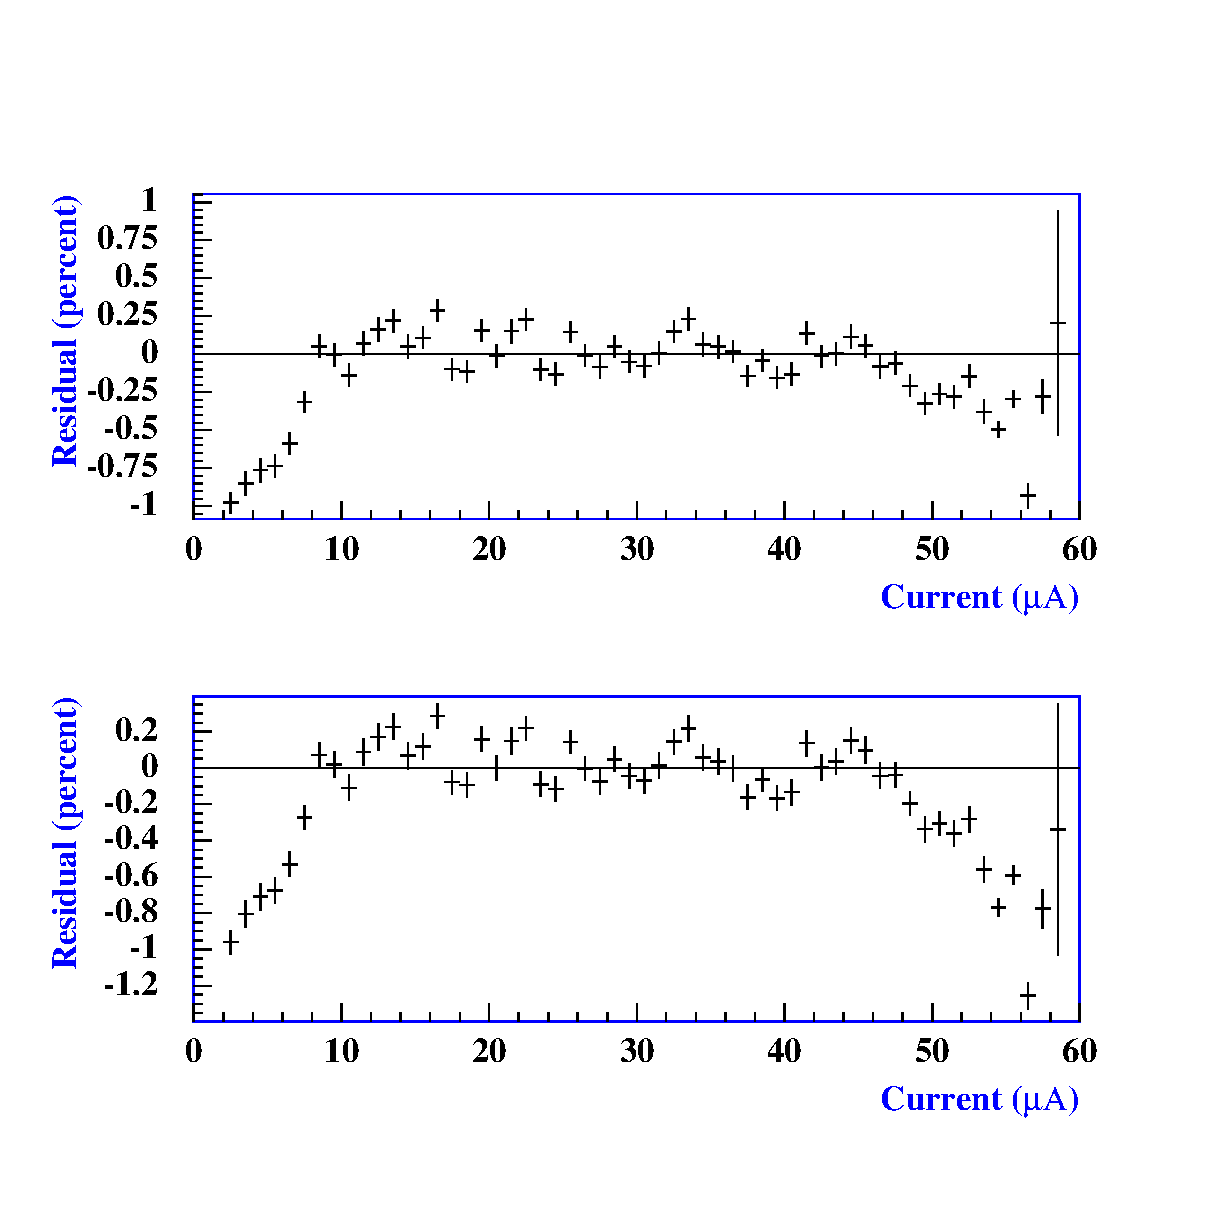
\includegraphics[width=3.5in]{DW/fig24_rsh_linearbu.eps}
\caption{(Color online) (top) Residuals from fit of BCM1 to Unser data, as a fraction
of the BCM1 pulse height at 32 $\mu$A, versus beam current.  (bottom)
Same for fit of BCM2 to Unser.}
% We need our own figure here.
\label{Fig24_RSH_Linearbu} 
\end{center}
\end{figure}

\begin{figure}
\begin{center}
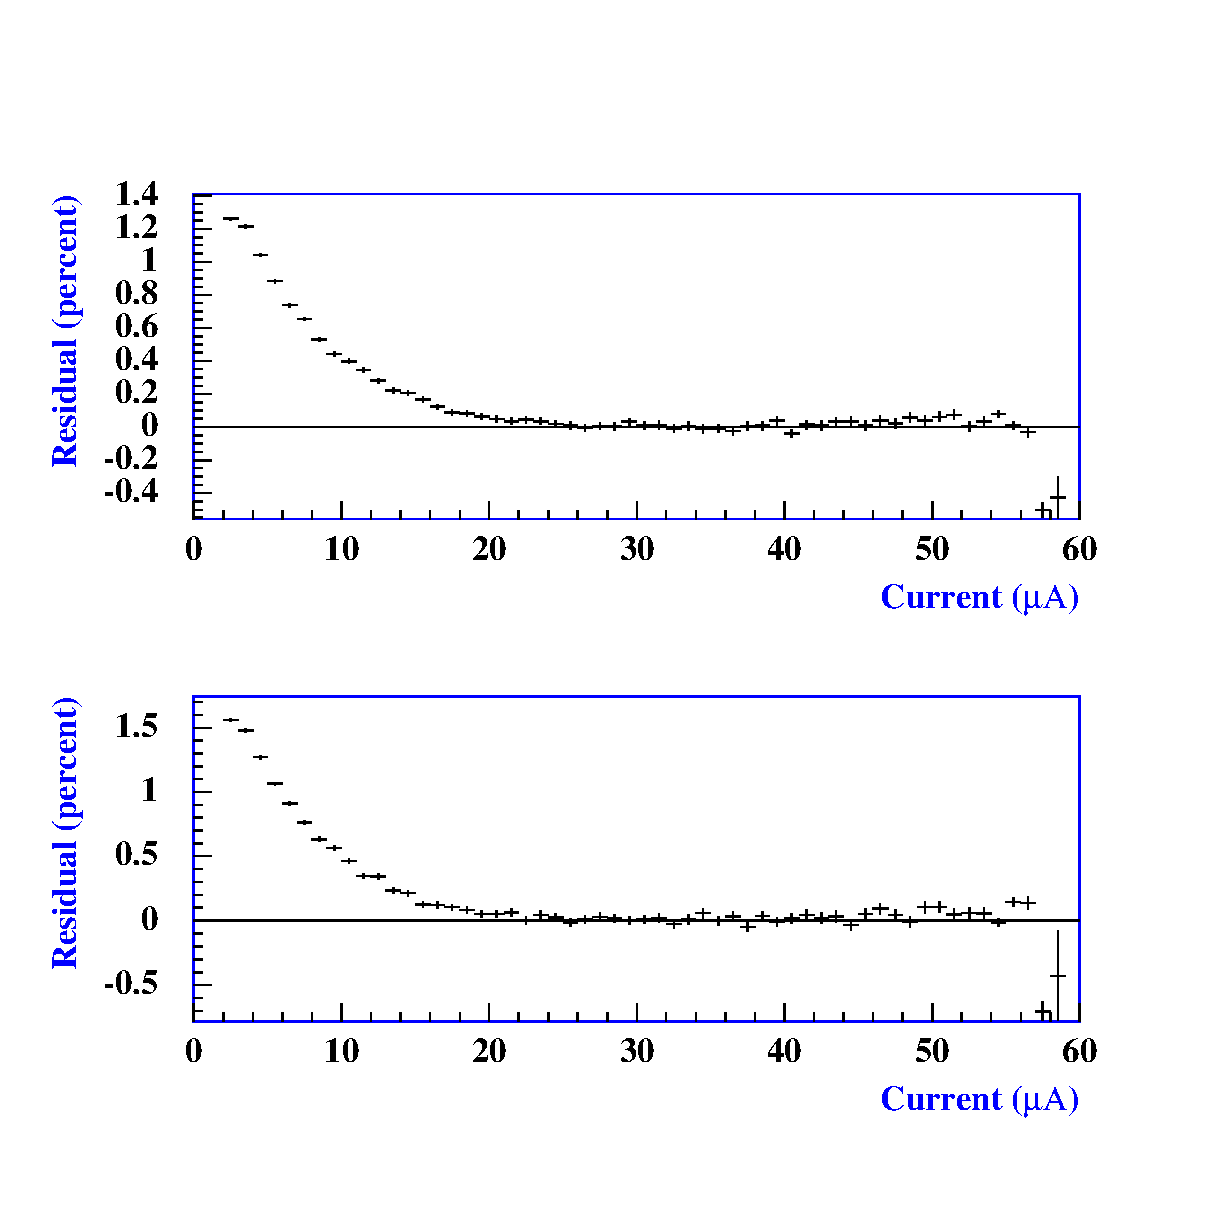
\includegraphics[width=3.5in]{DW/fig25_rsh_lineardb1.eps}
\caption{(Color online) (top) Residuals from fit of detector 1 to BCM1 data, as a fraction
of the detector 1 pulse height at 32 $\mu$A, versus beam current.  (bottom)
Same for fit of detector 2 to BCM1.}
% We need our own figure here.
\label{Fig25_RSH_Lineardb1} 
\end{center}
\end{figure}

Detector pedestals were measured by averaging the detector
signals during times when the beam is off.  The resulting pedestals
were always less than 0.3\% of the signal corresponding to the lowest
stable beam current in the production data set, and typically less
than 0.06\%; these pedestals are negligible.

The cavity monitor pedestals cannot be measured this way, since the
cavity signals are meaningless when the beam is off.  Instead, we fit
$I_{1(2)}$ to $I_U$ in the calibration data and extrapolate to zero
current.  Such an extrapolation requires knowledge of the average
Unser pedestal, which is obtained from the beam-off data in the same
run.  The resulting pedestals are less than 2\% of the signal
corresponding to the lowest stable beam current in the production data
set.

In conclusion, no corrections for pedestals or nonlinearities needed 
to be applied.  The nonlinearities of the detectors and cavity monitors
were negligible over the dynamic range of the beam current we ran.
The pedestals for detectors and cavity monitors were negligible.

\subsection{Systematic Fluctuations and Beam Corrections}
\label{sec:beamcorr}

Assuming that $\sigma(\asy_d)$ has negligible contributions from
window-to-window beam fluctuations and instrumentation noise,
there is still the possibility that there are 
helicity-correlated systematic effects at the sub-ppm
level. If one considers the cumulative corrected asymmetry
$\acorr_d$ over many window pairs, one can write
\begin{eqnarray}
\acorr_d & \equiv & \langle (\acorr_d)_i\rangle = 
\nonumber \\
&  & 
\left\langle\left(\frac{\Delta D}{2D}\right)_i\right\rangle -
\left\langle\left(\frac{\Delta I}{2I}\right)_i\right\rangle
- \sum_j {\beta_j\left\langle{(\Delta M_j)_i}\right\rangle} 
\nonumber \\
&=& \asy_D -  \asy_I - \sum_j \asy_{Mj}.
\end{eqnarray}

For most of the running conditions during data collection,
$\acorr_d\simeq \asy_D\simeq 10$~ppm, which meant that all
corrections were negligible. The cumulative average for $\asy_I$ was
maintained below 0.1 ppm. For $\asy_{Mj}$, the cumulative averages
were found to be below 0.1 ppm during the run with the ``bulk'' GaAs
photocathode. This resulted from the fact that the accelerator
damped out position fluctuations produced at the source by a large
factor (section \ref{sec:adiabatic_damp}). 
The averaged position differences 
on target were kept below 10 nm.

However, during data collection with ``strained'' GaAs, position
differences as large as several $\mu$m were observed in the
electron beam at a point in the accelerator where the beam energy is
5 MeV. Continuous adjustment of the circular polarization of the
laser beam was required to reduce the differences to about 0.5
$\mu$m. This resulted in observed position differences on target
ranging from 10 nm to 100 nm, which in turn resulted in $\asy_{Mj}$
in the range from 0.1 to 1 ppm.

The control of the asymmetry corrections within the aforementioned
constraints was one of the central challenges during data
collection. A variety of feedback techniques on the laser and
electron beam properties were employed in order to accomplish
this; these methods are discussed in Sec.~\ref{sec:laser}.

\input{KP/som_pid}

\subsection{Background Analysis}

\subsubsection{Target EndCap Correction}

Scattering from the target aluminum windows contributed
(0.5 $\pm$ 0.1)\% (???) to our detected signal.
This background was measured by 
inserting into the beam an empty
aluminum target cell, similar to the one used to
contain liquid deuterium, and measuring the 
signal in our detector. 
The thickness of the empty target cell walls is about 10 times
that of the walls used in the deuterium cell, in
order to compensate for the radiative
losses in the deuterium cell.  

The correction to our data arises from ... ??? ... explain the
physics here; I guess if it's DIS it's then Aluminum is
not much different from Deuterium ...


\subsubsection{Calibration of The HRS Optics}\label{sec:ana_optics}

To calibrate the transfer matrix for the HRS, a 0.5 mm thick 
tungsten plate with an array of pinholes
is inserted about 1 meter after the target and upstream
of the first quadrupole of the HRS.
The calibrations are dedicated runs at low rates with the
vertical drift chambers (VDCs) turned on.
Using the hole-pattern observed in the HRS focal plane,
a chi-square minimization algorithm is performed to 
determine the matrix elements which transform the
track vector to the location of the sieve slit.

Show some results from Kai Pan's analysis here.


\subsubsection{Reconstruction of $Q^2$ and $x$}\label{sec:ana_q2}

The four-momentum transfer squared is 
\begin{equation} \label{eq:qsq}
Q^2 \hskip 0.05in
= \hskip 0.05in 2 \hskip 0.02in E \hskip 0.02in 
E^{\prime} \hskip 0.02in (1- {\rm cos}(\theta))
\end{equation}
where $E$ is the incident energy, $E^{\prime}$ is the
final momentum or energy of the 
electron ($E^{\prime} \gg m_e$) and
$\theta$ is the scattering angle.  

For the beam energy we used the Tiefenbach energy (need to 
explain this) of ??? GeV
and assumed a 3 MeV (???) average energy loss to the center of the 
target which is applied
this as a correction to the beam energy.  
The error in the beam energy $E$ and $E^{\prime}$ are assumed
conservatively to be 3 MeV based on a history of these measurements
in Hall A.  The most important error is in $\theta$ ...

Perhaps need a table of errors.

%the following is copied from Bob's v1 but according to the new outline should be separated into two simulations. The HAMC should go into section ``Q2 reconstruction'' (above), the HATS should be a stand-alone subsection of ``Analysis''.

\subsection{Simulation}

Two simulation packages were used to support the analysis of this experiment.
The package called ``hamc'' (Hall A Monte Carlo) was used to simulate
the events and the spectrometer acceptance, while a second package
called ``hats'' (Hall A Trigger Simulation) was used to simulate the
response of the trigger used to identify electrons and pions, providing
a calculation of our deadtime.

In ``hamc'', events are generated using a physics class that has information about the cross section and asymmetry.  
The tracks are generated uniformly in solid angle 
\hskip 0.05in $d\Omega = sin(\theta) \hskip 0.02in d\theta \hskip 0.02in d\phi$ \hskip 0.05in and 
the results later weighted by the differential cross section $\frac{d\sigma}{d\Omega}$. 
The simulated tracks undergo multiple scattering in the target and 
energy loss from the target from external and internal Brehmstrahlung as 
well as ionization loss, 

The generated four-vectors are transported to the detector in the HRS focal plane using 
a set of polynomials that model the trajectories of electrons through the magnetic fields.
The beam raster is simulated, which produces a smearing of the beam on target.
The events are transported to intermediate apertures such as the collimator 
or the entrance to quadrupoles. 
Events that reach the HRS focal plane and intersect the detectors are integrated 
to compute the total rate and average asymmetry.

Here describe ``hats'' ...


\input{DW/som_radcor}
\input{DW/som_hats}

%Extraction of Results
\input{XZ/som_extraction}

% In setting up this template for *Science* papers, we've used both
% the \section* command and the \paragraph* command for topical
% divisions.  Which you use will of course depend on the type of paper
% you're writing.  Review Articles tend to have displayed headings, for
% which \section* is more appropriate; Research Articles, when they have
% formal topical divisions at all, tend to signal them with bold text
% that runs into the paragraph, for which \paragraph* is the right
% choice.  Either way, use the asterisk (*) modifier, as shown, to
% suppress numbering.

% Your references go at the end of the main text, and before the
% figures.  For this document we've used BibTeX, the .bib file
% scibib.bib, and the .bst file Science.bst.  The package scicite.sty
% was included to format the reference numbers according to *Science*
% style.

%
\input{XZ/som_summary}


%\bibliography{DW/pvdis_dw}
%\bibliography{RM/pvdis_rm}
%\bibliography{PR/pvdis_pr}
%\bibliography{KP/pvdis_kp}
%\bibliography{XZ/pvdis_xz}

%\bibliographystyle{Science}
\begin{thebibliography}{99} 
\input{DW/pvdis_bib_dw}

\bibitem{chargeden}B. Frois \etal, Phys. Rev. Lett. {\bf 38}, 152 (1977).
\bibitem{pions}C.~Garcia-Recio, J.~Nieves, E.~Oset,
 %``Neutron distributions from pionic atoms,''
 Nucl.\ Phys.\  A {\bf 547}, 473 (1992).
\bibitem{protons1} L. Ray, W. R. Coker, G.W. Hoffmann, Phys. Rev. C {\bf 18}, 2641 (1978).
\bibitem{protons2} V.E. Starodubsky, N.M. Hintz, Phys. Rev. C {\bf 49}, 2118 (1994).
\bibitem{protons3} B.C. Clark, L.J. Kerr, S. Hama, Phys. Rev. C {\bf 67}, 054605 (2003). 
\bibitem{antiprotons1} A. Trzcinska \etal, Phys. Rev. Lett. {\bf 87}, 082501 (2001).
\bibitem{antiprotons2} H. Lenske, Hyperfine Interact. {\bf 194}, 277 (2009).
\bibitem{dds} T.W. Donnelly, J. Dubach, I.~Sick, Nucl. Phys.A {\bf 503}, 589 (1989).
\bibitem{couldist} C.J. Horowitz, Phys. Rev. C {\bf 57} , 3430 (1998).
\bibitem{bigprex} C.J. Horowitz, S.J. Pollock, P.A. Souder, R. Michaels, Phys. Rev. C {\bf 63}, 025501 (2001).
%\bibitem{coldatomsMIT}Y. Shin \etal, Phys. Rev. Lett. {\bf 97}, 030401 (2006).
%\bibitem{coldatomsRICE}G.B. Partridge \etal, Science {\bf 311}, 503 (2006).

%nl3, nl3m05, nl3p06
%\cite{Lalazissis:1996rd}
\bibitem{Lalazissis:1996rd}
  G.A.~Lalazissis, J.~Konig, P.~Ring,
  %``A New parametrization for the Lagrangian density of relativistic mean 
%  field theory,''
  Phys.\ Rev.\ C {\bf 55}, 540 (1997).
%  arXiv:9607039 [nucl-th].

%fsu
%\cite{ToddRutel:2005zz}
\bibitem{ToddRutel:2005zz}
  B.G.~Todd-Rutel, J.~Piekarewicz,
  %``Neutron-Rich Nuclei and Neutron Stars: A New Accurately Calibrated
 % Interaction for the Study of Neutron-Rich Matter,''
  Phys.\ Rev.\ Lett.\  {\bf 95}, 122501 (2005).
  


%siii
%\cite{Beiner:1974gc}
\bibitem{Beiner:1974gc}
  M.~Beiner, H.~Flocard, N.~van Giai, P.~Quentin,
  %``Nuclear ground state properties and selfconsistent calculations with the
%  Skyrme interactions: 1. Spherical description,''
  Nucl.\ Phys.\  A {\bf 238}, 29 (1975).
 
%sty4
%\cite{Chabanat:1997un}
\bibitem{Chabanat:1997un}
  E.~Chabanat, P.~Bonche, P.~Haensel, J.~Meyer, R.~Schaeffer,
  %``A Skyrme parametrization from subnuclear to neutron star
 % densities. 2. Nuclei far from stablities,''
  Nucl.\ Phys.\ A {\bf 635}, 231 (1998).
  
%si
%\cite{Vautherin:1971aw}
\bibitem{Vautherin:1971aw}
  D.~Vautherin, D.~M.~Brink,
  %``Hartree-Fock calculations with Skyrme's interaction. 1. Spherical
 % nuclei,''
  Phys.\ Rev.\  C {\bf 5}, 626 (1972).
  

%\bibitem{prex} Jefferson Laboratory Exp. E-00-03, Spokespersons K. Kumar, R. Michaels, P.A. Souder, and G.M. Urcioli.
\bibitem{alexbrown}B.A.~Brown, Phys. Rev. Lett. {\bf 85}, 5296 (2000). 
\bibitem{rNSvsRn} C.J. Horowitz, J. Piekarewicz, Phys. Rev. {\bf C64}, 062802 (2001).
%\bibitem{MvsREOS}James M. Lattimer, Maddapa Prakash, Phys. Rept. {\bf 442}, 109 (2007). 
%\bibitem{lowmass}J. Carriere, C.J. Horowitz, J. Piekarewicz, Astrophys. J. {\bf 593}, 463 (2003).

\bibitem{Ozel:2010fw}
  F.~Ozel, G.~Baym, T.~Guver,
  %``Astrophysical Measurement of the Equation of State of Neutron Star Matter,''
  Phys.\ Rev.\  D {\bf 82}, 101301 (2010).
 % [arXiv:1002.3153 [astro-ph.HE]].

%\cite{Steiner:2010fz}
\bibitem{Steiner:2010fz}
  A.~W.~Steiner, J.~M.~Lattimer, E.~F.~Brown,
  %``The Equation of State from Observed Masses and Radii of Neutron Stars,''
  Astrophys.\ J.\  {\bf 722}, 33 (2010).
%  [arXiv:1005.0811 [astro-ph.HE]].
%A.~Steiner, J.~M.~Lattimer, E.~F.~Brown, arXiv:1005.0811.

%\cite{Hebeler:2010jx}
\bibitem{Hebeler:2010jx}
  K.~Hebeler, J.~M.~Lattimer, C.~J.~Pethick, A.~Schwenk,
  %``Constraints on neutron star radii based on chiral effective field theory interactions,''
  Phys.\ Rev.\ Lett.\  {\bf 105}, 161102 (2010).
%  [arXiv:1007.1746 [nucl-th]].

\bibitem{MC3n} %checked on inspire,not yet in print
S. Gandolfi, J. Carlson, S. Reddy, arXiv:1101.1921.

\bibitem{isospindif} {
W. G. Lynch \etal,
%M. B. Tsang, Y. Zhang, P. Danielewicz, M. Famiano, Z. Li, A. W. Steiner 
arXiv:0901.0412.}

\bibitem{isospindif2}M.B. Tsang \etal, 
%Yingxun Zhang, P.Danielewicz, M.Famiano, Zhuxia Li, W.G.Lynch, A.W.Steiner, 
Phys. Rev. Lett. {\bf 102}, 122701 (2009). 
\bibitem{URCA}C.J. Horowitz, J. Piekarewicz, Phys. Rev. C {\bf 66}, 055803 (2002). 
\bibitem{cjhjp_prl}C.J. Horowitz, J. Piekarewicz, Phys. Rev. Lett. {\bf 86},  5647 (2001).
\bibitem{Reinhard}P. G. Reinhard, W. Nazarewicz, Phys. Rev. C {\bf 81}, 051303 (2010).
\bibitem{tamii} A. Tamii et al., Phys. Rev. Lett. {\bf 107}, 062502 (2011).

\bibitem{Pollock} S.~J.~Pollock, E.~N.~Fortson, and L.~Wilets,
Phys. Rev. C {\bf 46}, 2587 (1992); S.J.~Pollock and M.C.~Welliver, Phys.
Lett. B {\bf 464}, 177 (1999)

\bibitem{brownAPV} B.A. Brown, A. Derevianko, V. V. Flambaum, Phys. Rev. C {\bf 79}, 035501 (2009).
%\bibitem{cesium} cesium APV.
\bibitem{berkeleyAPV}
K. Tsigutkin \etal, 
%D. Dounas-Frazer, A. Family, J. E. Stalnaker, V. V. Yashchuk, D. Budker, 
  Phys.\ Rev.\  A {\bf 81}, 032114 (2010).
%[arXiv:1001.0587].

%\cite{Acha:2006my}
\bibitem{Acha:2006my}
  A.~Acha \etal 
  %``Precision Measurements of the Nucleon Strange Form Factors at Q**2 ~
  %0.1-GeV**2,''
  Phys.\ Rev.\ Lett.\  {\bf 98}, 032301 (2007).
%  [arXiv:nucl-ex/0609002].
  %%CITATION = PRLTA,98,032301;%%

%\cite{Aniol:2005zf}
\bibitem{Aniol:2005zf}
  K.~A.~Aniol \etal  
  %``Parity-violating electron scattering from He-4 and the strange electric
  %form-factor of the nucleon,''
  Phys.\ Rev.\ Lett.\  {\bf 96}, 022003 (2006).
%  [arXiv:nucl-ex/0506010].
  %%CITATION = PRLTA,96,022003;%%

\bibitem{Aniol:PRC2004}
  K.~A.~Aniol \etal  
  Phys. Rev. C {\bf 69}, 065501 (2004). 

%\cite{Alcorn:2004sb}
\bibitem{Alcorn:2004sb}
  J.~Alcorn  % %B.~D.~Anderson, K.~A.~Aniol, J.~R.~M.~Annand, L.~Auerbach, J.~Arrington, T.~Averett, F.~T.~Baker 
 \etal,  %``Basic Instrumentation for Hall A at Jefferson Lab,''
  Nucl.\ Instrum.\ Meth.\ A {\bf 522}, 294 (2004).
%Hall A collaboration,\journal{Nucl. Instr. Meth.}{A522}{294-346}{2004}.
%

\bibitem{Sinclair2007}
C. K. Sinclair, {\it et.al.} Phys. Rev. ST Accel. Beams 10, 023501 (2007);
J. Hansknecht, {\it et.al.} Phys. Rev. ST Accel. Beams 13, 010101 (2010).

%
%\cite{Paschke:2007zz}
\bibitem{Paschke:2007zz}
  K.~D.~Paschke,
  %``Controlling helicity-correlated beam asymmetries in a polarized electron source,''
  Eur.\ Phys.\ J.\  A {\bf 32}, 549 (2007).

\bibitem{Ong} A. Ong, J. C. Berengut, V. V. Flambaum, Phys. Rev. C {\bf 82}, 014320 (2010).

%\cite{Ban:2010wx}
\bibitem{Ban:2010wx}
  S.~Ban, C.J.~Horowitz, R.~Michaels,
  %``Parity Violating Electron Scattering Measurements of Neutron Densities,''
J. Phys G {\bf 39} (2012) 015104.


%\cite{RocaMaza:2011pm}
\bibitem{RocaMaza:2011pm}
  X.~Roca-Maza, M.~Centelles, X.~Vinas, M.~Warda,
  %``Neutron skin of $^{208}Pb$, nuclear symmetry energy, and the parity radius
  %experiment,''
Phys. Rev. Lett. {\bf 106}, 252501 (2011).
%[arXiv:1103.1762 [nucl-th]].



\input{PR/pvdis_bib_pr}
\input{KP/pvdis_bib_kp}
\input{XZ/pvdis_bib_xz}
\end{thebibliography}



% Following is a new environment, {scilastnote}, that's defined in the
% preamble and that allows authors to add a reference at the end of the
% list that's not signaled in the text; such references are used in
% *Science* for acknowledgments of funding, help, etc.

\begin{scilastnote}
\item 
We would like to thank the personnel of Jefferson Lab for their efforts which 
resulted in the successful completion of the experiment.
We thank T.-S.H.~Lee, M.~Gorshteyn, P.~Blunden, A.~Afanasev, J. Erler 
and their collaborators for carrying out the calculations used in this publication (list all
theorists not co-author-ed here). 
X.~Zheng would like to thank the Medium Energy Physics Group at the Argonne National 
Lab for supporting her during the initial work of this experiment. 
This work was supported by the Department of Energy (DOE), 
the National Science Foundation,
%the Italian Istituto Nazionale di Fisica Nucleare,
%the French Institut National de Physique Nucl\'{e}aire et de Physique des Particules,
%the French Commissariat \`{a} l'\'{E}nergie Atomique
and the Jeffress Memorial Trust. 
Jefferson Science Associates, LLC,  operates Jefferson Lab for the U.S. DOE under U.S. DOE 
contract DE-AC05-060R23177.
\end{scilastnote}




% For your review copy (i.e., the file you initially send in for
% evaluation), you can use the {figure} environment and the
% \includegraphics command to stream your figures into the text, placing
% all figures at the end.  For the final, revised manuscript for
% acceptance and production, however, PostScript or other graphics
% should not be streamed into your compliled file.  Instead, set
% captions as simple paragraphs (with a \noindent tag), setting them
% off from the rest of the text with a \clearpage as shown  below, and
% submit figures as separate files according to the Art Department's
% instructions.


%%%\clearpage

%%%\noindent {\bf Fig. 1.} Please do not use figure environments to set
%%%up your figures in the final (post-peer-review) draft, do not include graphics in your
%%%source code, and do not cite figures in the text using \LaTeX\
%%%\verb+\ref+ commands.  Instead, simply refer to the figure numbers in
%%%the text per {\it Science\/} style, and include the list of captions at
%%%the end of the document, coded as ordinary paragraphs as shown in the
%%%\texttt{scifile.tex} template file.  Your actual figure files should
%%%be submitted separately.



\end{document}




















